% Options for packages loaded elsewhere
\PassOptionsToPackage{unicode}{hyperref}
\PassOptionsToPackage{hyphens}{url}
\PassOptionsToPackage{dvipsnames,svgnames,x11names}{xcolor}
%
\documentclass[
  letterpaper,
  DIV=11,
  numbers=noendperiod]{scrreprt}

\usepackage{amsmath,amssymb}
\usepackage{lmodern}
\usepackage{iftex}
\ifPDFTeX
  \usepackage[T1]{fontenc}
  \usepackage[utf8]{inputenc}
  \usepackage{textcomp} % provide euro and other symbols
\else % if luatex or xetex
  \usepackage{unicode-math}
  \defaultfontfeatures{Scale=MatchLowercase}
  \defaultfontfeatures[\rmfamily]{Ligatures=TeX,Scale=1}
\fi
% Use upquote if available, for straight quotes in verbatim environments
\IfFileExists{upquote.sty}{\usepackage{upquote}}{}
\IfFileExists{microtype.sty}{% use microtype if available
  \usepackage[]{microtype}
  \UseMicrotypeSet[protrusion]{basicmath} % disable protrusion for tt fonts
}{}
\makeatletter
\@ifundefined{KOMAClassName}{% if non-KOMA class
  \IfFileExists{parskip.sty}{%
    \usepackage{parskip}
  }{% else
    \setlength{\parindent}{0pt}
    \setlength{\parskip}{6pt plus 2pt minus 1pt}}
}{% if KOMA class
  \KOMAoptions{parskip=half}}
\makeatother
\usepackage{xcolor}
\setlength{\emergencystretch}{3em} % prevent overfull lines
\setcounter{secnumdepth}{5}
% Make \paragraph and \subparagraph free-standing
\ifx\paragraph\undefined\else
  \let\oldparagraph\paragraph
  \renewcommand{\paragraph}[1]{\oldparagraph{#1}\mbox{}}
\fi
\ifx\subparagraph\undefined\else
  \let\oldsubparagraph\subparagraph
  \renewcommand{\subparagraph}[1]{\oldsubparagraph{#1}\mbox{}}
\fi


\providecommand{\tightlist}{%
  \setlength{\itemsep}{0pt}\setlength{\parskip}{0pt}}\usepackage{longtable,booktabs,array}
\usepackage{calc} % for calculating minipage widths
% Correct order of tables after \paragraph or \subparagraph
\usepackage{etoolbox}
\makeatletter
\patchcmd\longtable{\par}{\if@noskipsec\mbox{}\fi\par}{}{}
\makeatother
% Allow footnotes in longtable head/foot
\IfFileExists{footnotehyper.sty}{\usepackage{footnotehyper}}{\usepackage{footnote}}
\makesavenoteenv{longtable}
\usepackage{graphicx}
\makeatletter
\def\maxwidth{\ifdim\Gin@nat@width>\linewidth\linewidth\else\Gin@nat@width\fi}
\def\maxheight{\ifdim\Gin@nat@height>\textheight\textheight\else\Gin@nat@height\fi}
\makeatother
% Scale images if necessary, so that they will not overflow the page
% margins by default, and it is still possible to overwrite the defaults
% using explicit options in \includegraphics[width, height, ...]{}
\setkeys{Gin}{width=\maxwidth,height=\maxheight,keepaspectratio}
% Set default figure placement to htbp
\makeatletter
\def\fps@figure{htbp}
\makeatother
\newlength{\cslhangindent}
\setlength{\cslhangindent}{1.5em}
\newlength{\csllabelwidth}
\setlength{\csllabelwidth}{3em}
\newlength{\cslentryspacingunit} % times entry-spacing
\setlength{\cslentryspacingunit}{\parskip}
\newenvironment{CSLReferences}[2] % #1 hanging-ident, #2 entry spacing
 {% don't indent paragraphs
  \setlength{\parindent}{0pt}
  % turn on hanging indent if param 1 is 1
  \ifodd #1
  \let\oldpar\par
  \def\par{\hangindent=\cslhangindent\oldpar}
  \fi
  % set entry spacing
  \setlength{\parskip}{#2\cslentryspacingunit}
 }%
 {}
\usepackage{calc}
\newcommand{\CSLBlock}[1]{#1\hfill\break}
\newcommand{\CSLLeftMargin}[1]{\parbox[t]{\csllabelwidth}{#1}}
\newcommand{\CSLRightInline}[1]{\parbox[t]{\linewidth - \csllabelwidth}{#1}\break}
\newcommand{\CSLIndent}[1]{\hspace{\cslhangindent}#1}

\KOMAoption{captions}{tableheading}
\makeatletter
\makeatother
\makeatletter
\@ifpackageloaded{bookmark}{}{\usepackage{bookmark}}
\makeatother
\makeatletter
\@ifpackageloaded{caption}{}{\usepackage{caption}}
\AtBeginDocument{%
\ifdefined\contentsname
  \renewcommand*\contentsname{Table of contents}
\else
  \newcommand\contentsname{Table of contents}
\fi
\ifdefined\listfigurename
  \renewcommand*\listfigurename{List of Figures}
\else
  \newcommand\listfigurename{List of Figures}
\fi
\ifdefined\listtablename
  \renewcommand*\listtablename{List of Tables}
\else
  \newcommand\listtablename{List of Tables}
\fi
\ifdefined\figurename
  \renewcommand*\figurename{Figure}
\else
  \newcommand\figurename{Figure}
\fi
\ifdefined\tablename
  \renewcommand*\tablename{Table}
\else
  \newcommand\tablename{Table}
\fi
}
\@ifpackageloaded{float}{}{\usepackage{float}}
\floatstyle{ruled}
\@ifundefined{c@chapter}{\newfloat{codelisting}{h}{lop}}{\newfloat{codelisting}{h}{lop}[chapter]}
\floatname{codelisting}{Listing}
\newcommand*\listoflistings{\listof{codelisting}{List of Listings}}
\makeatother
\makeatletter
\@ifpackageloaded{caption}{}{\usepackage{caption}}
\@ifpackageloaded{subcaption}{}{\usepackage{subcaption}}
\makeatother
\makeatletter
\@ifpackageloaded{tcolorbox}{}{\usepackage[many]{tcolorbox}}
\makeatother
\makeatletter
\@ifundefined{shadecolor}{\definecolor{shadecolor}{rgb}{.97, .97, .97}}
\makeatother
\makeatletter
\makeatother
\ifLuaTeX
  \usepackage{selnolig}  % disable illegal ligatures
\fi
\IfFileExists{bookmark.sty}{\usepackage{bookmark}}{\usepackage{hyperref}}
\IfFileExists{xurl.sty}{\usepackage{xurl}}{} % add URL line breaks if available
\urlstyle{same} % disable monospaced font for URLs
\hypersetup{
  pdftitle={GUTS RDM Handbook},
  pdfauthor={Mark Mulder, Eduard Klapwijk},
  colorlinks=true,
  linkcolor={blue},
  filecolor={Maroon},
  citecolor={Blue},
  urlcolor={Blue},
  pdfcreator={LaTeX via pandoc}}

\title{GUTS RDM Handbook}
\author{Mark Mulder, Eduard Klapwijk}
\date{1/6/23}

\begin{document}
\maketitle
\ifdefined\Shaded\renewenvironment{Shaded}{\begin{tcolorbox}[boxrule=0pt, borderline west={3pt}{0pt}{shadecolor}, breakable, enhanced, interior hidden, sharp corners, frame hidden]}{\end{tcolorbox}}\fi

\renewcommand*\contentsname{Table of contents}
{
\hypersetup{linkcolor=}
\setcounter{tocdepth}{2}
\tableofcontents
}
\bookmarksetup{startatroot}

\hypertarget{welcome}{%
\chapter*{Welcome}\label{welcome}}
\addcontentsline{toc}{chapter}{Welcome}

\markboth{Welcome}{Welcome}

This is the website for the \textbf{Research Data Management (RDM)
Handbook} of the \textbf{Growing Up Together in Society (GUTS)}
consortium.

The goal of the GUTS RDM Handbook is to bring everything about data
collection, data management, and data handling in the GUTS consortium
together in a central and easily searchable place. First and foremost,
the goal is to facilitate data management within the GUTS consortium.
Second, we hope that this handbook might be useful for other projects.
We are building upon resources and wisdom of many others, we hope to pay
it forward by making this resource openly available.

The GUTS consortium investigates youth from the perspective of societal
neuroscience, and combines insights and expertise from neuroscience,
psychology, psychiatry, and sociology. The consortium is funded by a
Gravitation grant from the Ministry of Education, Culture and Science
for a ten-year period (2023-2033). To learn more about GUTS visit
\url{https://growinguptogetherinsociety.com/}.

\part{Why invest in RDM?}

The first part of this handbook provides background on why it is
important to invest time and resources in Research Data Management in a
project like GUTS.

\hypertarget{the-benefits-of-good-rdm}{%
\chapter{The benefits of good RDM}\label{the-benefits-of-good-rdm}}

\href{https://the-turing-way.netlify.app/afterword/glossary.html\#term-Research-Data-Management}{Research
Data Management} (RDM) considers the organisation, storage and
preservation of data created during a research project. It covers a wide
range of activities such as initial planning, day-to-day processes and
long-term archiving and sharing. This means that the list of benefits of
doing this well is quite extensive as well. Here we provide a
non-exhaustive list of benefits:

\begin{itemize}
\item
  proper data storage and backup prevents data loss
\item
  making data understandable for others (and your future self) allows
  reuse and collaboration
\item
  proper data management is key to Open Science, since transparency and
  reuse of data is only possible using well-documented data
\item
  good RDM also helps to prevent misconduct since it helps to show the
  integrity of the data collection process
\item
  it makes research go more smoothly, allowing you as a researcher to
  focus on the problems of science rather than data administravia
  (Briney, Coates, and Goben 2020)
\end{itemize}

\hypertarget{fair-data}{%
\chapter{FAIR data}\label{fair-data}}

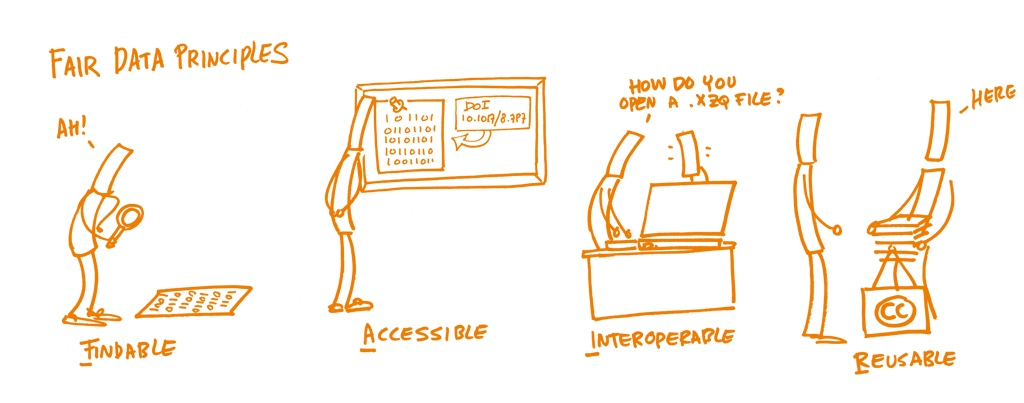
\includegraphics{https://www.ugent.be/img/doza/beleid/rdm/fair-data.png}

Picture: \href{https://www.ugent.be/img/doza/beleid/fair-data.png}{FAIR
principles} / Patrick Hochstenbach /
\href{https://creativecommons.org/publicdomain/zero/1.0/}{CC0 1.0}

\hypertarget{data-management-planning}{%
\chapter{Data management planning}\label{data-management-planning}}

\part{Data collection}

\hypertarget{how-to-save-your-data}{%
\chapter{How to save your data}\label{how-to-save-your-data}}

\href{https://the-turing-way.netlify.app/afterword/glossary.html\#term-Research-Data-Management}{Research
Data Management} (RDM) considers the organisation, storage and
preservation of data created during a research project. It covers a wide
range of activities such as initial planning, day-to-day processes and
long-term archiving and sharing. This means that the list of benefits of
doing this well is quite extensive as well. Here we provide a
non-exhaustive list of benefits:

\begin{itemize}
\item
  proper data storage and backup prevents data loss
\item
  making data understandable for others (and your future self) allows
  reuse and collaboration
\item
  proper data management is key to Open Science, since transparency and
  reuse of data is only possible using well-documented data
\item
  good RDM also helps to prevent misconduct since it helps to show the
  integrity of the data collection process
\item
  it makes research go more smoothly, allowing you as a researcher to
  focus on the problems of science rather than data administravia
  (Briney, Coates, and Goben 2020)
\end{itemize}

\hypertarget{data-formats}{%
\chapter{Data formats}\label{data-formats}}

\hypertarget{metadata}{%
\chapter{Metadata}\label{metadata}}

\hypertarget{guts-codebook}{%
\chapter{GUTS codebook}\label{guts-codebook}}

\begin{longtable}[]{@{}
  >{\raggedright\arraybackslash}p{(\columnwidth - 12\tabcolsep) * \real{0.0938}}
  >{\raggedright\arraybackslash}p{(\columnwidth - 12\tabcolsep) * \real{0.1406}}
  >{\raggedright\arraybackslash}p{(\columnwidth - 12\tabcolsep) * \real{0.1094}}
  >{\raggedright\arraybackslash}p{(\columnwidth - 12\tabcolsep) * \real{0.2109}}
  >{\raggedright\arraybackslash}p{(\columnwidth - 12\tabcolsep) * \real{0.1562}}
  >{\raggedright\arraybackslash}p{(\columnwidth - 12\tabcolsep) * \real{0.1250}}
  >{\raggedright\arraybackslash}p{(\columnwidth - 12\tabcolsep) * \real{0.1250}}@{}}
\toprule()
\begin{minipage}[b]{\linewidth}\raggedright
name
\end{minipage} & \begin{minipage}[b]{\linewidth}\raggedright
label
\end{minipage} & \begin{minipage}[b]{\linewidth}\raggedright
data\_type
\end{minipage} & \begin{minipage}[b]{\linewidth}\raggedright
value\_labels
\end{minipage} & \begin{minipage}[b]{\linewidth}\raggedright
measurement units
\end{minipage} & \begin{minipage}[b]{\linewidth}\raggedright
minimum value
\end{minipage} & \begin{minipage}[b]{\linewidth}\raggedright
maximum value
\end{minipage} \\
\midrule()
\endhead
age & age in years & numeric & & years:months & 0 & 116 \\
education & education level & categorical &
\begin{minipage}[t]{\linewidth}\raggedright
\begin{enumerate}
\def\labelenumi{\arabic{enumi}.}
\setcounter{enumi}{-1}
\tightlist
\item
  missing
\item
  in high school
\item
  finished high school
\item
  some college
\item
  college graduate
\item
  graduate degree
\end{enumerate}
\end{minipage} & & & \\
\bottomrule()
\end{longtable}

\hypertarget{file-naming}{%
\chapter{File naming}\label{file-naming}}

Good and structured file names will help you and your collaborators to
easily navigate the content and status of files in your project. Within
the GUTS consortium we use file naming conventions from the Brain
Imaging Data Structure (BIDS) for MRI and related files. For all other
files, we suggest the following best practices:

In general, good file names are (see also Klapwijk (2023)):

\begin{itemize}
\item
  Machine-readable:

  \begin{itemize}
  \item
    Use not much more than letters, numbers, hyphens and underscores.
    Avoid spaces, punctuation, accented characters, and case sensitivity

    \begin{itemize}
    \tightlist
    \item
      For example, \texttt{paper\_flanker-task\_draft01.docx} is
      preferred over \texttt{paper\ “flanker\ task”\ draft01(1).docx}
    \end{itemize}
  \item
    Deliberately use delimiters. Use a hyphen (-) to mean "different
    words that are part of the same chunk", and underscore (\_) to
    separate different chunks of metadata

    \begin{itemize}
    \tightlist
    \item
      For example, file names in the
      \href{https://bids.neuroimaging.io/}{BIDS specification} nicely
      follow this principle: the file
      \texttt{sub-01\_ses-02\_task-feedback\_run-01.nii} contains
      instances of the ``subject'', ``ses(sion)'', ``task'' an ``run''
      entities, making it evident from the filename alone that it
      contains the \texttt{nii} (nifti) feedback task data for run
      \texttt{01} from session \texttt{02} of subject \texttt{01}
    \end{itemize}
  \end{itemize}
\item
  Human-readable:

  \begin{itemize}
  \item
    Good file names provide useful clues to the content, status and
    version of a file, uniquely identify a file and help in classifying
    and sorting files
  \item
    Choose keywords and file names that are sufficiently descriptive,
    e.g.,
    \texttt{analysis01\_descriptive-statistics.R},\texttt{analysis02\_preregistered-analysis.R}
  \end{itemize}
\item
  Make sorting and searching easy:

  \begin{itemize}
  \item
    Use YYYY-MM-DD date format (ISO 8601 standard)
  \item
    To order files put date or number first, e.g.,
    \texttt{2019-01-01\_original-analysis.R},
    \texttt{2019-12-01\_minor-changes-to-original.R},
    \texttt{01\_original-analysis.R},
    \texttt{02\_minor-changes-to-original.R}
  \item
    Include the version of the file, e.g.,
    \texttt{methodology-section\ \_v1}
  \end{itemize}
\end{itemize}

\bookmarksetup{startatroot}

\hypertarget{glossary}{%
\chapter*{Glossary}\label{glossary}}
\addcontentsline{toc}{chapter}{Glossary}

\markboth{Glossary}{Glossary}

\hypertarget{sec-a}{%
\section*{A}\label{sec-a}}
\addcontentsline{toc}{section}{A}

\markright{A}

\textbf{Accessible}

One of the FAIR principles: Once a user finds the required data, they
need to know how data can be accessed, possibly including authentication
and authorisation.

\begin{center}\rule{0.5\linewidth}{0.5pt}\end{center}

\hypertarget{sec-b}{%
\section*{B}\label{sec-b}}
\addcontentsline{toc}{section}{B}

\markright{B}

\textbf{BIDS}

BIDS is the \href{https://bids.neuroimaging.io/}{Brain Imaging Data
Structure}. The specification is intentionally based on simple file
formats and folder structures to reflect current lab practices and make
it accessible to a wide range of scientists coming from different
backgrounds.

\begin{center}\rule{0.5\linewidth}{0.5pt}\end{center}

\hypertarget{sec-g}{%
\section*{G}\label{sec-g}}
\addcontentsline{toc}{section}{G}

\markright{G}

\textbf{GUTS}

The GUTS (Growing Up Together in Society) consortium investigates youth
from the perspective of societal neuroscience, and combines insights and
expertise from neuroscience, psychology, psychiatry, and sociology. The
consortium is funded by a Gravitation grant from the Ministry of
Education, Culture and Science for a ten-year period (2023-2033). To
learn more about GUTS visit
\href{https://growinguptogetherinsociety.com/}{the GUTS consortium
website}

\begin{center}\rule{0.5\linewidth}{0.5pt}\end{center}

\hypertarget{sec-r}{%
\section*{R}\label{sec-r}}
\addcontentsline{toc}{section}{R}

\markright{R}

\textbf{Research Data Management}

Research Data Management (RDM) considers the organisation, storage and
preservation of data created during a research project. It covers a wide
range of activities such as initial planning, day-to-day processes and
long-term archiving and sharing.

\bookmarksetup{startatroot}

\hypertarget{references}{%
\chapter*{References}\label{references}}
\addcontentsline{toc}{chapter}{References}

\markboth{References}{References}

\hypertarget{refs}{}
\begin{CSLReferences}{1}{0}
\leavevmode\vadjust pre{\hypertarget{ref-briney2020}{}}%
Briney, Kristin, Heather Coates, and Abigail Goben. 2020.
{``Foundational Practices of Research Data Management.''} \emph{Research
Ideas and Outcomes} 6 (July): e56508.
\url{https://doi.org/10.3897/rio.6.e56508}.

\leavevmode\vadjust pre{\hypertarget{ref-klapwijk2023}{}}%
Klapwijk, Eduard. 2023. {``Best Practices for Documenting and Organizing
Research Projects,''} January.
\url{https://doi.org/10.5281/ZENODO.7551576}.

\end{CSLReferences}



\end{document}
